\chapter{Introduction}\label{chapter:Introduction}
\epigraph{Saving our planet, lifting people out of poverty, advancing economic growth... these are one and the same fight. We must connect the dots between climate change, water scarcity, energy shortages, global health, food security and women's empowerment. Solutions to one problem must be solutions for all.}{\textit{Ban Ki-moon}}

This dissertation considers a way to solve the global problems of energy shortage and environment problem.

\section{Research background and significance}
% 现有太阳能光热发电技术简析,提出太阳能梯级发电的背景及其意义。
% 能源和环境现状

% 太阳能光热发电现状
% 文献1
Concentrating solar power technologies use different mirror configurations to concentrate the sun's light energy onto a receiver and convert it into heat. The heat can then be used to create steam to drive a turbine to produce electrical power or used as industrial process heat.

Concentrating solar power plants can integrate thermal energy storage systems to generate electricity during cloudy periods or even several hours after the sunset. CSP systems can be also combined with combined cycle power plants resulting in hybrid power plants which provide high-value, dispatch-able power. These attributes, make concentrating solar power the most attractive renewable energy option in the Sunbelt regions.

There are four types of CSP technologies being applied. For each of these, there are various design variations or different configurations.

%文献2
In addition to wind and photovoltaic power, concentrating solar thermal power (CSP) will make a major contribution to electricity provision from renewable energies. Drawing on almost 30 years of operational experience in the multi-megawatt range, CSP is now a proven technology with a reliable cost and performance record. In conjunction with thermal energy storage, electricity can be provided according to demand. To date, solar thermal power plants with a total capacity of 1.3 GW are in operation worldwide, with an additional 2.3 GW under construction and 31.7 GW in advanced planning stage. Depending on the concentration factors, temperatures up to 1000°C can be reached to produce saturated or superheated steam for steam turbine cycles or compressed hot gas for gas turbine cycles. The heat rejected from these thermodynamic cycles can be used for sea water desalination, process heat and centralized provision of chilled water. While electricity generation from CSP plants is still more expensive than from wind turbines or photovoltaic panels, its independence from fluctuations and daily variation of wind speed and solar radiation provides it with a higher value. To become competitive with mid-load electricity from conventional power plants within the next 10–15 years, mass production of components, increased plant size and planning/operating experience will be accompanied by technological innovations. On 30 October 2009, a number of major industrial companies joined forces to establish the so-called DESERTEC Industry Initiative, which aims at providing by 2050 15 per cent of European electricity from renewable energy sources in North Africa, while at the same time securing energy, water, income and employment for this region. Solar thermal power plants are in the heart of this concept.
% 梯级发电的意义

\section{State of the art}
% 范围的大小
%国内外对太阳能光热发电技术的研究现状。
%外文文献-问题-解决方案-本项目需求

\subsection{Solar Parabolic Trough}\label{sec:pt}

Parabolic trough solar technology is the most proven and lowest cost large-scale solar power technology available.~\cite{Price2002}

Figure~\ref{fig:pt} shows a parabolic trough product made by Alpha-E.

\begin{figure}[!ht]
\centering
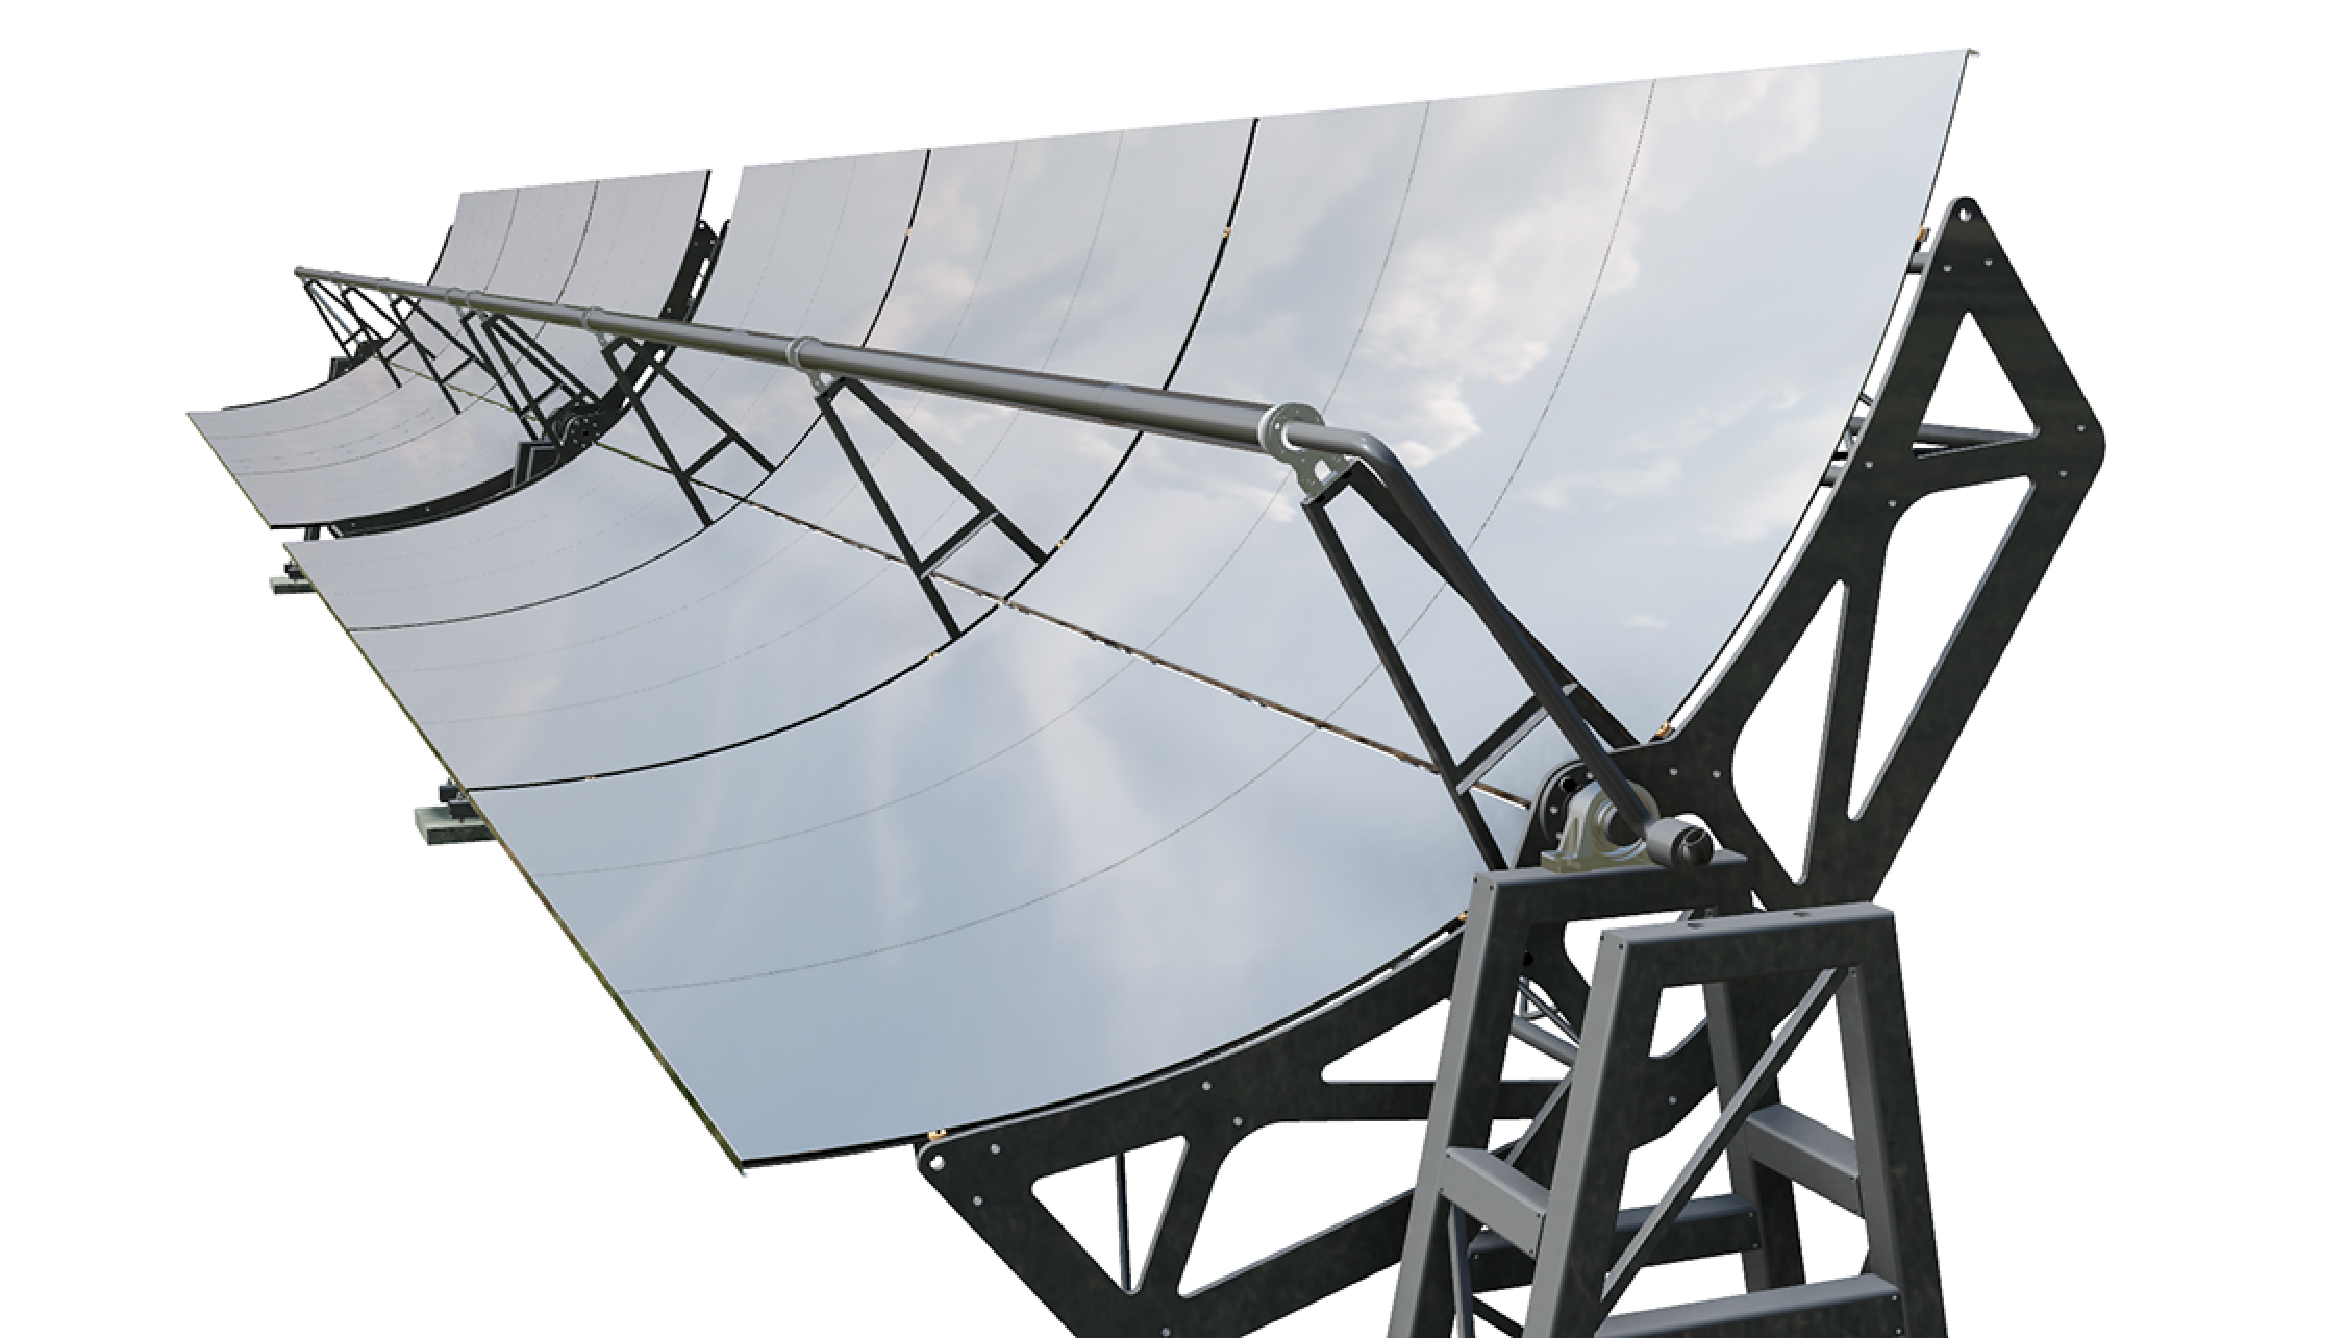
\includegraphics[width=.7\textwidth]{fig/ParabolicTrough.png}
\caption{Alpha-Trough-350, a parabolic trough product made by Alpha-E}\label{fig:pt}
\end{figure}

Padilla~\cite{Padilla2011} performed a detailed one dimensional numerical heat transfer analysis of a PTC (Parabolic Trough Collector). To solve the mathematical model of heat transfer of the PTC model, the partial differential equations were discretized and the nonlinear algebraic equations were solved simultaneously. The numerical results was validated to the data from Sandia National Laboratory (SNL).
\nomenclature[C]{PTC}{Parabolic Trough Collector}
\nomenclature[C]{SNL}{Sandia National Laboratory}

To understand the thermal performance of the collector and identify the heat losses from the collector, Mohamad~\cite{Mohamad2014} analyzed the temperature variation of the working fluid, tube and glass along the collector.

Guo~\cite{JiangfengGuo2016-1} investigated the energy efficiency and exergy efficiency of the parabolic trough collector. The result shown that there exists an optimal mass flow rate of working fluid for exergy efficiency, and the thermal efficiency and exergy efficiency have opposite changing tendencies under some conditions.

Guo~\cite{JiangfengGuo2016-2} implemented a multi-parameter optimization of parabolic trough solar receiver based on genetic algorithm where Exergy and thermal efficiencies were employed as objective function.

Padilla~\cite{Padilla2014} performed a comprehensive exergy balance of a parabolic trough collector based on the previous heat transfer model~\cite{Padilla2011}. The results shown that inlet temperature of heat transfer fluid, solar irradiance, and vacuum in annulus have a significant effect on the thermal and exergetic performance, but the effect of wind speed and mass flow rate of heat transfer fluid is negligible. It was obtained that inlet temperature of heat transfer fluid cannot be optimized to achieve simultaneously maximum thermal and exergetic efficiency because they exhibit opposite trends. Finally, it was found that the highest exergy destruction is due to the heat transfer between the sun and the absorber while for exergy losses is due to optical error.

Huang~\cite{Huang2012} proposed an analytical model for optical performance which employed a modified integration algorithm.

Wang~\cite{Wang2016} proposed a mathematical model for the optical efficiency of the parabolic trough solar collector and selected three typical regions of solar thermal utilization in China for the model. The model is validated by comparing the test results in parabolic trough power plant, with relative error range of 1\% to about 5\%.

Al-Sulaiman~\cite{AlSulaiman2014} presented the exergy analysis of selected thermal power systems driven by PTSCs. The power pf the thermal power system is produced using either a steam Rankine cycle (SRC) or a combined cycle, in which the SRC is the topping cycle and an organic Rankine cycle (ORC) is the bottoming cycle.
\nomenclature[C]{SRC}{Steam Rankine Cycle}
\nomenclature[C]{ORC}{Organic Rankine Cycle}

Hachicha~\cite{Hachicha2013} presented a detailed numerical heat transfer model based on the finite volume method for the parabolic trough collector.  This model is based on finite volume method and ray trace techniques and takes into account the finite size of the Sun.  The model is thoroughly validated with results from the literature and it shows a good agreement with experimental and analytical results.

Ashouri~\cite{Ashouri2015} coupled a small scale parabolic trough collector and a thermal storage tank along with an auxiliary heater to a Kalina cycle to study the performance of the system throughout the year, both thermodynamically and economically.

Guo~\cite{SuGuo2016} developed a nonlinear distribution parameter model to model the dynamic behaviors of direct steam generation parabolic trough collector loops under either full or partial solar irradiance disturbance.

Bader~\cite{Bader2015} developed a numerical model of a tubular vavity-receiver that uses air as the heat transfer fluid. Four different receiver configurations are considered, with smooth or V-corrugated absorber tube and single- or double-glazed aperture window. The different types of energy loss by the collector have been quantified, and the temperature distribution inside the receiver has been studied. The pumping power required to pump the HTF through the receiver has been determined for a 200 m long collector row.

Good~\cite{Good2015} proposed solar trough concentrators using air as heat transfer fluid at operating temperatures exceeding $600\,^\circ$C. It consists of an array of helically coiled absorber tubes contained side-by-side within an insulated groove having a rectangular windowed opening. Secondary concentrating optics are incorporated to boost the geometric concentration ratio to 97$\times$.

Boukelia~\cite{Boukelia2016} investigated the feed-forward back-propagation learning algorithm with three different variants; Levenberge Marguardt (LM), Scaled Conjugate Gradient (SCG), and Pola-Ribiere Conjugate Gradient (PCG), used in artificial neural network (ANN) to find the best approach for prediction and techno-economic optimization of parabolic trough solar thermal power plant (PTSTPP) integrated with fuel backup system and thermal energy storage.
\nomenclature[C]{LM}{Levenberge Marguardt}
\nomenclature[C]{SCG}{Scaled Conjugate Gradient}
\nomenclature[C]{PCG}{Pola-Ribiere Conjugate Gradient}
\nomenclature[C]{ANN}{Artificial Neural Network}
\nomenclature[C]{PTSTPP}{Parabolic Trough Solar Thermal Power Plant}

Kaloudis~\cite{Kaloudis2016} investigated a PTC system with nanofluid as the HTF in terms of Computational Fluid Dynamics (CFD). Syltherm 800 liquid oil was used as the HTF, and Al$_2$O$_3$ nanoparticles with the concentrations ranges from 0\% to 4\% was investigated. A boost up to 10\% on the collector efficiency was reported for Al$_2$O$_3$ concentration of 4\%.
\nomenclature[C]{HTF}{Heat Transfer Fluid}
\nomenclature[C]{CFD}{Computational Fluid Dynamics}

Tan~\cite{Tan2014} proposed a two-stage photovoltaic thermal system based on solar trough concentration is proposed, in which the metal cavity heating stage is added on the basis of the PV/T stage, and thermal energy with higher temperature is output while electric energy is output. The experimental platform of the two-stage photovoltaic thermal system was established, with a 1.8 m$^2$ mirror PV/T stage and a 15 m$^2$ mirror heating stage, or a 1.8 m$^2$ mirror PV/T stage and a 30 m$^2$ mirror heating stage. The results showed that with single cycle, the long metal cavity heating stage would bring lower thermal efficiency, but temperature rise of the working medium is higher, up to 12.06$^\circ$C with only single cycle. With 30 min closed multiple cycles, the temperature of the working medium in the water tank was 62.8$^\circ$C, with an increase of 28.7$^\circ$C, and thermal energy with higher temperature could be output.

Al-Sulaiman~\cite{AlSulaiman2012} proposed a novel system based on PTC and ORC for combined cooling, heating and power (CCHP). Performance assessment, including efficiency, net electrical power, and electrical to heating and cooling ratios, of the system shown that when CCHP is used, the efficiency increases significantly. This study reveals that the maximum electrical efficiency for the solar mode is 15\%, for the solar and storage mode is 7\%, and for the storage mode is 6.5\%. The maximum CCHP efficiency for the solar mode is 94\%, for the solar and storage mode is 47\%, and for the storage mode is 42\%.
\nomenclature[C]{CCHP}{Combined cooling, heating and power}

Lobon~\cite{Lobon2014} introduced a computational fluid dynamic simulation approach to predict the behavior of a solar steam generating system, which is located at the Plataforma Solar de Almeria, Spain. The CFD package STAR-CCM+ code has been used to implement an efficient multiphase model capable of simulating the dynamics of the multiphase fluid in parabolic-trough solar collectors. Numerical and experimental data are compared in a wide range of working conditions.
\nomenclature[C]{DSG}{Direct Steam Generation}

Xu~\cite{Xu2014} presented a method to compensate the end loss effect of PTC. An optical analysis on the end loss effect of PTC with horizontal north-south axis (PTC-HNSA) is performed and a five-meter PTC-HNSA experimental system was built. The increased thermal efficiency of the experimental system is measured, and the result that the experimental value (increased thermal efficiency) substantially agreed with the theoretical value (increased optical efficiency) is gained.

Liu~\cite{Liu2012} developed a mathematical model of PTC using the least squares support vector machine (LSSVM) method. Numerical simulations are implemented to evaluate the feasibility and efficiency of the LSSVM method, where the sample data derived from the experiment and the simulation results of two solar collector systems with 30 m$^2$ and 600 m$^2$ solar fields, and the complicated relationship between the solar collector efficiency and the solar flux, the flow rate and the inlet temperature of the heat transfer fluid (HTF) is extracted.
\nomenclature[C]{LSSVM}{Least squares support vector machine}

\subsection{Solar Parabolic dish}\label{sec:pd}

One of the main goals of the BIOSTIRLING-4SKA project, funded by the European Commission, is the development of a hybrid Dish-Stirling system based on a hybrid solar-gas receiver, which has been designed by the Swedish company Cleanergy.~\cite{Blazquez2016}

Craig~\cite{Craig2016b} proposed two types of cooking sections of the solar parabolic dish system: the spiral hot plate copper tube and the heat pipe plate. A conical cavity of copper tubes were put on the focus of the collectors to collect heat and the heat is stored inside an insulated tank which acts both as storage and cooking plate. The use of heat pipes to transfer heat between the oil storage and the cooking pot was compared to the use of a direct natural syphon principle which is achieved using copper tubes in spiral form like electric stove. An accurate theoretical analysis for the heat pipe cooker was achieved by solving the boiling and vaporization in the evaporator side and then balancing it with the condensation and liquid-vapor interaction in the condenser part while correct heat transfer, pressure and height balancing was calculated in the second experiment. The results show and compare the cooking time, boiling characteristics, overall utilization efficiencies and necessary comparison between the two system and other existing systems.

Flux distribution of the receiver is simulated successfully by Mao~\cite{Mao2014b} using MCRT method. The impacts of incident solar irradiation, aspect ratio (the ratio of the receiver height to the receiver diameter), and system error on the radiation flux of the receiver are investigated.
\nomenclature[C]{MCRT}{Monte Carlo Ray Tracing}

Mawire~\cite{Mawire2014} investigated the thermal performance of a cylindrical cavity receiver for an SK-14 parabolic dish concentrator. The receiver exergy rates and efficiencies are found to be appreciably smaller than the receiver energy rates and efficiencies. The exergy factor is found to be high under conditions of high solar radiation and under high operating temperatures. An optical efficiency of around 52\% for parabolic dish system is determined under high solar radiation conditions.

Reddy~\cite{Reddy2015,Reddy2015_2} performed the theoretical thermal performance analysis of a fuzzy focal solar parabolic dish concentrator with modified cavity receiver. Total heat loss from the modified cavity receiver is estimated considering the effects of wind conditions, operating temperature, emissivity of the cavity cover and thickness of insulation. Time constant test was carried out to determine the influence of sudden change in solar radiation at steady state conditions. The daily performance tests were conducted for different flow rates.

Vikram~\cite{Vikram2015} investigated the total heat losses of modified cavity receiver of SPD with three configurations using 3D numerical model. The effects of various parameters such as diameter ratio, angle of inclination, operating temperature, insulation thickness and emissivity of the cavity cover on the heat losses from the modified vavity receiver are investigated. An ANN model is developed to predict the heat loss for a large set of influencing parameters. Based on ANN modeling, improved Nusselt number correlations are proposed for convective, radiative and total heat losses from the modified cavity receiver. The convective heat losses are greatly influenced by receiver inclination whereas the radiation heat losses are influenced by the cavity cover emissivity. The diameter ratio also plays a major role in heat losses from the cavity receiver. The present method predicts the heat losses more accurately compared with the existing models.

Atul~\cite{Atul2015} proposed a low-cost solar dish water heating system and investigated the effect of variation of mass flow rate on performance of the heater prototype. A novel truncated cone-shaped helical coiled receiver made up of copper is put at the focal point of SP.

CRTEn developed a solar parabolic concentrator (SPC) using four types of absorbers: flat plat, disk, water calorimeter and solar heat exchanger.~\cite{Skouri2013} For the system different types of absorbers, experiments were conducted to obtain the mean concentration ratio and both energy and exergy efficiency. Results shown that thermal energy efficiency of the system varies from 40\% to 77\%, the concentrating system reaches an average exergy efficiency of 50\% and a concentration factor around 178.
\nomenclature[C]{CRTEn}{Research and Technologies Centre of Energy in Borj Cedria}
\nomenclature[C]{SPC}{Solar parabolic concentrator}

Blazquez~\cite{Blazquez2016} studied the optimization of the concentrator and receiver cavity geometry of parabolic dish system. Ray-tracing analysis has been performed with the open source software Tonatiuh, a ray-tracing tool specifically oriented to the modeling of solar concentrators.

Uma~\cite{Uma2015} carried out the simulation of the structural, thermal and CFD analysis of the dish with varying metallic properties (Aluminium, Copper and StainlessSteel) under different wind conditions. Computational Fluid Dynamics (CFD) was done to simulate the thermal performance of the dish at two different wind velocities.

Patil~\cite{Patil2016} described the development of automatic dual axis solar tracking system for solar parabolic dish. Five light dependent resistors were used to sense the sunlight and Two permanent magnet DC motors are used to move the solar dish. A controller software were developed to control the motors using the data sensed by the resistors.

Pavlovic~\cite{Pavlovic2014} presented a procedure to design a square facet concentrator for laboratory-scale research on medium-temperature thermal processes. A parabolic collector made up of individual square mirror panels (facets) were investigated. These facets can deliver up to 13.604 kW radiative power over a 250 mm radius disk (receiver) with average concentrating ratio exceeding 1200.

\subsection{Solar Tower}\label{sec:st}

Besarati and Yogi~\cite{Besarati2014} A number of codes have been developed in order to optimize the heliostat field layout for solar power tower plants. These codes are intended to improve calculation accuracy as well as computational time. Of all the factors that need to be taken into account in these codes, shading and blocking calculations introduce significant complexity as they are computationally intensive. In this paper, a new and simple method is proposed to identify the heliostats with the greatest potential for shadowing and blocking a heliostat. Using the new method, the computational time is considerably reduced as unnecessary calculations are avoided. The Sassi method is then used to calculate the shading and blocking efficiency. The results are compared with the literature and good agreement is obtained. As a case study, the paper also investigates optimization of a 50 MWth heliostat field layout for Dagget, California. Yearly insolation weighted efficiency is selected as the objective function while two parameters of the prophylaxis pattern, which define the shape of the field layout, are the design variables. The acceptance angle of the cavity receiver and distance between the adjacent heliostats are the physical constraints which are included in the optimization. The optimization algorithm is explained in detail and the optimal field layout is presented.

Haroun~\cite{El2015} The aim of this work was to propose a novel system combines both solar chimney and thermo siphon solar tower systems. To this end, theoretical study to the proposed system was conducted. In this new system, the solar tower was installed at the exit of the solar chimney. The results of the theoretical study showed that, the new system generates more power compared with the conventional system. It was found that the maximum power extracted from the new system was about two times that obtained from the conventional system at the same height, for the specified range studied in this work. In addition, it was found that the new system has higher overall efficiency and generates higher speeds of air at the chimney inlet. This increase in both maximum power and air speed at the chimney inlet from the new system is enhanced with the rise in solar irradiance, radius of collector, and ratio of solar tower height to solar chimney height. Moreover, the results indicated that there is a certain ratio between solar tower length and width at which the maximum extracted mechanical power reached a maximum value for the specified parameters of solar irradiance, collector radius, height of chimney, and height of solar tower.

Franchini et al.~\cite{Franchini2013} Simulations were carried out to predict the performance of a Solar Rankine Cycle (SRC) and an Integrated Solar Combined Cycle (ISCC) when combined with two different solar field configurations based on parabolic trough and power tower systems. For the selected cases, yearly plant performance was computed under real operating conditions on a one hour basis. A computing procedure was developed by integrating two commercial softwares with in-house computer code. Thermodynamic performance was featured for every plant configuration both at nominal and part load conditions. A single reheat regenerative Rankine cycle was chosen for the \{SRC\} plant whereas a commercial gas turbine, i.e. Siemens SGT-800, with a dual pressure heat recovery steam generator (HRSG) was assumed for the \{ISCC\} plant. As far as the heat transfer fluid (HTF) is concerned, molten salt was chosen to transfer heat to the water loop in the SRC. Synthetic oil was considered in the \{ISCC\} plant. Plants were assumed to be located in a Southern Spain site. The comparative analysis was mainly focused on the influence of \{CSP\} technology on global solar energy conversion efficiency of both \{SRC\} and \{ISCC\} plants. Special attention was devoted to assess trough collectors (PTCs) against the solar tower (ST) system in terms of intercepted radiation and thermal power sent to the power block. The \{ISCC\} coupled with a \{ST\} was found to assure the highest annual solar-to-electric efficiency of 21.8\%. This is the result of both higher collection efficiency of \{ST\} compared to \{PTCs\} and higher conversion efficiency of solar energy introduced into the combined cycle, as compared to SRC.


Kim et al.~\cite{Kim2015} Heat loss is an important factor in predicting the performance of solar receiver of concentrated solar power (CSP) systems. This study presents a numerical simulation calculating convection and radiation heat losses from four different receiver shapes including external and cavity type receivers with different opening ratios (ratio of cavity aperture area to receiver area). The simulation was carried out using Fluent \{CFD\} (computational fluid dynamics) software considering three different receiver temperatures (600, 750, and 900 $\,^{\circ}$C), three wind velocities (1, 5, and 10 m/s), and two wind directions (head-on and side-on). The simulation results were then used for deriving a simplified correlation model which gives the fraction of convection heat loss by a function of opening ratio, receiver temperature, and wind velocity. The calculated fraction can be easily converted to convection heat loss, total heat loss, or receiver efficiency once the radiation heat loss is estimated by any applicable prediction model. Calculated heat loses by the proposed simple correlation model showed good agreements with the simulation results with 11.4\% and 5.9\% average absolute deviations for convection heat loss and total heat loss, respectively. Validation of the model with experimental data was also carried out using test results available from three central receiver systems (Martin Marietta, Solar One and Solar Two).

Lara et al.~\cite{Lara2016} A novel modeling tool for calculation of central receiver concentrated flux distributions is presented, which takes into account drift effects. This tool is based on a drift model that includes different geometrical error sources in a rigorous manner and on a simple analytic approximation for the individual flux distribution of a heliostat. The model is applied to a group of heliostats of a real field to obtain the resulting flux distribution and its variation along the day. The distributions differ strongly from those obtained assuming the ideal case without drift or a case with a Gaussian tracking error function. The time evolution of peak flux is also calculated to demonstrate the capabilities of the model. The evolution of this parameter also shows strong differences in comparison to the case without drift.

Ramos~\cite{Ramos2012} A method for optimizing a central receiver solar thermal electric power plant is studied. We parametrize the plant design as a function of eleven design variables and reduce the problem of finding optimal designs to the numerical problem of finding the minimum of a function of several variables. This minimization problem is attacked with different algorithms both local and global in nature. We find that all algorithms find the same minimum of the objective function. The performance of each of the algorithms and the resulting designs are studied for two typical cases. We describe a method to evaluate the impact of design variables in the plant performance. This method will tell us what variables are key to the optimal plant design and which ones are less important. This information can be used to further improve the plant design and to accelerate the optimization procedure.

Wei et al.~\cite{Wei2010} A new method for the design of the heliostat field layout for solar tower power plant is proposed. In the new method, the heliostat boundary is constrained by the receiver geometrical aperture and the efficiency factor which is the product of the annual cosine efficiency and the annual atmospheric transmission efficiency of heliostat. With the new method, the annual interception efficiency does not need to be calculated when places the heliostats, therefore the total time of design and optimization is saved significantly. Based on the new method, a new code for heliostat field layout design (HFLD) has been developed and a new heliostat field layout for the PS10 plant at the PS10 location has been designed by using the new code. Compared with current PS10 layout, the new designed heliostats have the same optical efficiency but with a faster response speed. In addition, to evaluate the feasibility of crops growth on the field land under heliostats, a new calculation method for the annual sunshine duration on the land surface is proposed as well. ?? 2010 Elsevier Ltd. All rights reserved.

Wei et al.~\cite{Wei2010a} A new code for the design and analysis of the heliostat field layout for power tower system is developed. In the new code, a new method for the heliostat field layout is proposed based on the edge ray principle of nonimaging optics. The heliostat field boundary is constrained by the tower height, the receiver tilt angle and size and the heliostat efficiency factor which is the product of the annual cosine efficiency and the annual atmospheric transmission efficiency. With the new method, the heliostat can be placed with a higher efficiency and a faster response speed of the design and optimization can be obtained. A new module for the analysis of the aspherical heliostat is created in the new code. A new toroidal heliostat field is designed and analyzed by using the new code. Compared with the spherical heliostat, the solar image radius of the field is reduced by about 30{\%} by using the toroidal heliostat if the mirror shape and the tracking are ideal. In addition, to maximize the utilization of land, suitable crops can be considered to be planted under heliostats. To evaluate the feasibility of the crop growth, a method for calculating the annual distribution of sunshine duration on the land surface is developed as well.

Xu et al.~\cite{Xu2011a} 1 MW Dahan solar thermal power tower plant is modeled from mathematical models for all of the working conditions using the modular modeling method. The dynamic and static characteristics of the power plant are analyzed based on these models. Response curves of the system state parameters are given for different solar irradiance disturbances. Conclusions in this paper are good references for the design of solar thermal power tower plant.

Xu et al.~\cite{Xu2012} In this paper, the thermal energy storage system of Badaling 1 MW solar power tower plant is modelled from mathematical models for whole of the working conditions using the modular modelling method. This model can accurately simulate the recharge and discharge processes of thermal energy storage system. The dynamic and static characteristics of the thermal energy storage system are analyzed based on the model response curves of the system state parameters that are obtained from different steam flow disturbances. Conclusions of this paper are good references for the design, operating, and control strategy of solar thermal power plant.

\subsection{Rankine Cycle}\label{sec:rc}



\subsection{Stirling Engine}\label{sec:se}

A large number of studies have been done on Stirling engine analysis. To describe a Stirling engine's behavior precisely is a difficult task due to the various losses and irreversibilities in the engine.
%Recent investigations~\cite{Tlili2006,Li2016} have found that these losses and irreversibilities in the thermodynamic cycle have significant importance in predicting the performance of Stirling engines.
Researchers have done a lot of work to build a precise Stirling engine model. Different models of Stirling engines were developed using empirical~\cite{Senft1998,Costea1999,Prieto2003,Organ2013,Kongtragool2005,Thombare2008}, analytical~\cite{Ohtomo1995,Rogdakis2004,Kongtragool2006,Puech2011,Formosa2010,Shazly2014,Cullen2011,Ahmadi2013,Ahmadi2013b,Tursunbaev2007} and numerical methods~\cite{Urieli1984,Ni2016,Jia2016,Strauss2010,Abbas2014,Araoz2015,Babaelahi2015,Barreto2017,Wu1998,Li2011,Hosseinzade2015}.

Among these methods, numerical methods obtain the most accurate models. Urieli and Berchowitz~\cite{Urieli1984} proposed an adiabatic model of Stirling engine considering some irreversible effects such as non-ideal heat transfer processes and pressure drop effect using numerical methods. The model is known as Simple model. Many researchers developed more accurate models based on the Simple model by using alternative methods or including more loss mechanisms.
Ni et al.~\cite{Ni2016} proposed an improved Simple analytical model which considers the influence mechanism of rotary speed, pressure and working gas in the view of heat/power losses for Stirling engine performance.
Jia et al.~\cite{Jia2016} developed a numerical model of free-piston engine generator. The dynamic equations have been linearized to simplify the model to a one-degree forced vibration system with various damping. The solving time of the proposed fast response model can be significantly reduced comparing to previous numerical models.
Strauss and Dobson~\cite{Strauss2010} proposed an alternative method to calculate the regeneration heat loss and pumping losses, which is more suitable for preliminary engine design and optimization, known as Simple II model.
Abbas~\cite{Abbas2014} considered the effects of non-ideal regeneration, shuttle loss and heat conduction losses based on Simple model.
Araoz et al.~\cite{Araoz2015} developed a rigorous Stirling engine model with adiabatic working spaces, isothermal heat exchangers. It considers dead volumes, and imperfect regeneration, mechanical pumping losses due to friction, limited heat transfer and thermal losses on the heat exchangers. The model is suitable for different engine configurations ($\alpha$, $\beta$ and $\gamma$ engines).
Babaelahi and Syyaadi~\cite{Babaelahi2015} proposed a new numerical thermal model based on polytropic expansion/compression processes. Differential equations in the expansion/compression processes were modified to polytropic processes in the new model. New model shows a better performance prediction compared with previous models.

With the development of finite-time thermodynamics, many researchers studied the the finite-time thermodynamic performance of the Stirling engine. This analysis can also be used in the case of irreversible machines further considering the internal irreversibilities of a Stirling engine such as friction, pressure drop and entropy generation~\cite{Barreto2017}.
Wu et al.~\cite{Wu1998} developed a numerical model considering finite-time effect to find out the relationship between the net power output and thermal efficiency of the engine.
Li et al.~\cite{Li2011} developed a mathematical model of a high temperature differential dish-Stirling system with finite-time thermodynamics. Finite-rate heat transfer, regenerative heat losses, conductive thermal bridging losses and finite regeneration processes of the Stirling engine were considered in the model.
Hosseinzade~\cite{Hosseinzade2015} presented a new closed-form thermal model for the thermal simulation of Stirling engines based on the combination of polytropic analysis of expansion/compression processes and the concept of finite speed thermodynamics.
Instead of finite-time method, Ahmadi et al.~\cite{Ahmadi2016b} proposed a finite-speed thermodynamic analysis based on the first law of thermodynamics for a closed system with finite speed and the direct method. The effects of heat source temperature, regenerating effectiveness, volumetric ratio, piston stroke as well as rotational speed are included in the analysis.
Chen et al.~\cite{Chen2007} developed a heat-engine cycle model using finite-time thermodynamics. The model, considered the losses due to heat-resistance, heat leaks and internal irreversibility, is applicable for generalized irreversible universal steady-flow heat-engine cycles.
%Cullen~\cite{Cullen2011} developed a theoretical Stirling engine model by using decoupled engine configuration in which working space swept volume, volume variation, phase angle and dead space ratio are controlled via a black-box electronic controller.

%Thombare~\cite{Thombare2008} presented a detailed review of the past methods and techniques used for engine analysis. Analysis of heat transfer phenomenon in the engine was also included in the review. Formosa~\cite{Formosa2010} developed an analytical model to predict the periodic steady operation under isothermal assumption and simplified heat transfer model. The model was validated using the experimental data of the General Motor GPU-3 Stirling engine prototype. Ohtomo~\cite{Ohtomo1995} proposed a simple graphic vector analysis method for the first-order estimation of the theoretical performance of Stirling engine with Schmidt assumption and, for simplicity, approximates all volume and pressure fluctuations as sinusoidal. Rogdakis~\cite{Rogdakis2004} used a linearization technique of the dynamic balance equations to predict the thermodynamic conditions for stable operation of free piston Stirling engines. Costea~\cite{Costea1999} considered the effects of both internal and external irreversibilities of the cycle. According to his research, the real cycle efficiency is approximately half the ideal cycle efficiency when the engine is operated at the optimum temperature. Araoz~\cite{Araoz2015} investigated the possible causes that limited the performance of a Stirling engine. Based on a second order Stirling engine model developed and validated previously, he implemented an analysis with the integration of thermodynamics, and the thermal and mechanical interactions of kinematic Stirling engines. Wu~\cite{Wu1998} built a model of Stirling engine with heat transfer and imperfect regeneration irreversibilities and derived the relationship between net power output and thermal efficiency by the model. Puech~\cite{Puech2011} and Kongtragool~\cite{Kongtragool2006} considered the influence of dead volume and imperfect regeneration on Stirling engine. An isothermal model was used to analyze the net work and the heat stored in the regenerator during a complete cycle. An analytical expression to estimate the improvement due to the regenerator has been proposed including the combined effects of dead volume and imperfect regeneration.  Formosa~\cite{Formosa2011} developed and validated an analytical thermodynamic model which encompasses the effectiveness and the flaws of the heat exchangers and the regenerator.

On the other side of the researches, multi-objective optimization algorithms were used considering multi-variables to obtain a better performance was paid for attention by numbers of researchers recently~\cite{Ahmadi2016,Li2016b,Patel2016,Luo2016}.
Ahmadi et al.~\cite{Ahmadi2016} performed the thermodynamic analysis of solar dish Stirling engine based on the finite-time thermodynamics. Then the NSGA-II algorithm was applied. Three objectives, thermal efficiency, entransy loss rate and power output, were set as the objectives and three well known decision making methods have been employed in the algorithm.
Li et al.~\cite{Li2016b} developed a multi-objective optimization model of a solar energy powered gamma type Stirling engine using Finite Physical Dimensions Thermodynamics (FPDT) method by multi-objective criteria. Genetic algorithm was used to get the Pareto frontier, and optimum points were obtained using the decision different making methods. Results show that total thermal conductance, hot temperature, stroke and diameter ratios can be improved.
Patel and Savsani~\cite{Patel2016} developed a strategy for multi-objective optimization for Stirling engines using TS-TLBO (tutorial training and self learning inspired teaching-learning-based optimization) algorithm. An application example with eleven decision variables and three objectives are considered.
Luo et al.~\cite{Luo2016} proposed a multiple optimization method that combines multiple optimization algorithms including differential evolution, genetic algorithm and adaptive simulated annealing. The optimization considers five decision variables, including engine frequency, mean effective pressure, temperature of heating source, number of wires in regenerator matrix, and the wire diameter of regenerator for maximum efficiency and output power.
\subsection{Brayton Cycle}\label{bc}
\section{Research Objective}\label{sec:3}
% 改进点,重点,难度
\section{Research Methods}
% 技术路线
